\documentclass[10pt]{article}
\usepackage{float}
\usepackage{listings}
\usepackage[french]{babel}
\usepackage[utf8x]{inputenc}
\usepackage{subcaption}
\usepackage{listings}
\usepackage{wrapfig}
\usepackage{color}
\usepackage{amsmath}
\usepackage{amsfonts}
\usepackage{mathtools}
\usepackage{graphicx}
\usepackage{caption}
\definecolor{dkgreen}{rgb}{0,0.6,0}
\definecolor{gray}{rgb}{0.5,0.5,0.5}
\definecolor{mauve}{rgb}{0.58,0,0.82}
%opening

\lstset
{frame=tb,
	language=R,
	aboveskip=3mm,
	belowskip=3mm,
	showstringspaces=false,
	framexleftmargin=5mm,
	columns= fixed,
	numbers = left,
	basicstyle={\small\ttfamily},	
	numberstyle=\tiny\color{gray},
	keywordstyle=\color{blue},
	commentstyle=\color{dkgreen},
	stringstyle=\color{mauve},
	breaklines=true,
	breakatwhitespace=true,
	tabsize=3
}


\title{
	\normalfont \normalsize 
	\textsc{Université de Technologie de Compiègne\\ 
		SY09:Analyse des données et Data-Mining , P17} \\
	[10pt] 
	\rule{\linewidth}{0.5pt} \\[6pt] 
	\huge Rendu TP2\\
	\rule{\linewidth}{2pt}  \\[10pt]
}
\author{Oumaima Talouka, Zineb Slam}
\date{\normalsize \today}

\begin{document}
	{\let\newpage\relax\maketitle}	
	
		Dans ce TP2 nous allons travailler sur la méthode de classification automatique qui est une  méthode non supervisée; c'est à dire nous  n'avons à priori aucune connaissance  sur le nombre ni sur le nom des classes qui peuvent exister. Nous utiliserons en majorité la méthode des centres mobiles dont nous analyserons et critiquerons les résultats
	
	\section{ Exercice 1: Visualisation des données}
	Nous disposons de 3 jeux de données:  \textbf{Iris}, \textbf{Crabs} et un jeu de données \textbf{Mutations} de dissimilarites des espèces
	
	\subsection{Iris}
		Les iris est un jeu de donnes de la librairie \textit{MASS} avec \textbf{150 individus} et 4 variables (Sepal.Length, Sepal.Width, Petal.Length et Petal.Width).  La variable Z de réponse est l'espèce d'appartenance. Le but est d'identifier l'espèce de chaque individu en fonction des 4 variables. Pour commencer nous allons centrer et réduire les données puis effectuer une ACP pour pourvoir réduire la dimension du dataset et passer de 4 dimensions à 2 dimensions. Après avoir fait appel à la fonction \textit{prcomp} nous affichons les données dans le premier plan factoriel sans tenir compte de l'espèce. Nous notons d'abord que les 2 premiers plan factoriels expliquent \textbf{95.8\%} des données \textit{(inertie expliquée}).  Ensuite  nous utilisons la fonction \textit{autoplot} pour colorer chaque individus selon son appartenance à une espèce et ce dans le même plan factoriel.
		
	
			\begin{minipage}{.5\textwidth}
			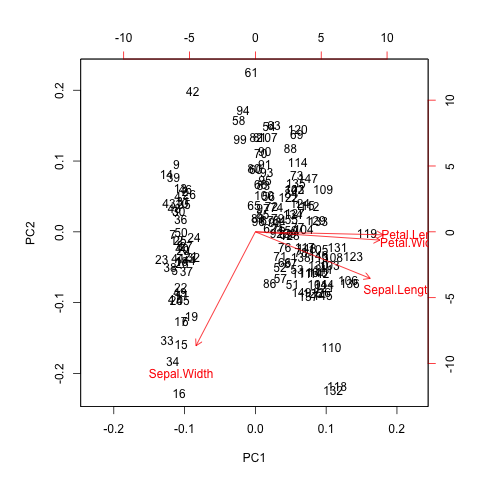
\includegraphics[width=45mm]{Figures/Iris_1/plotnospieces.png}
			\captionof{figure}{Représentation des Iris dans les 2 premiers plan factoriel}
			\label{fig:plot_iris_nocol}
		\end{minipage}%
		\hspace{0.02\linewidth}
		\begin{minipage}{.5\textwidth}
			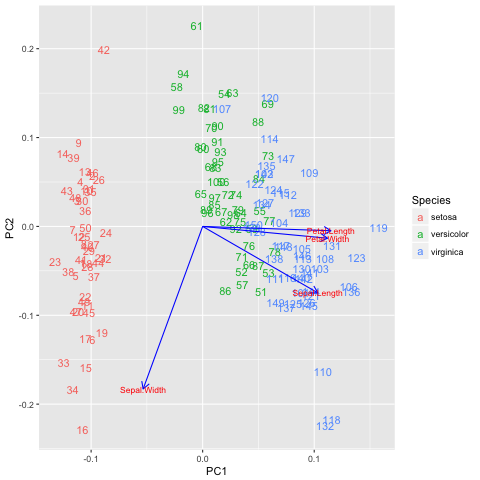
\includegraphics[width=45mm]{Figures/Iris_1/plotspieces.png}
		\captionof{figure}{Représentation des Iris dans les 2 premiers plan factoriel en colorant les espèces}
		\label{fig:plot_iris}
		\end{minipage}
		\vspace{0.2mm}
		
	 
		Nous observons donc que selon la figure  \ref{fig:plot_iris_nocol} qu'il existe au moins 2 classes bien distinctes. Néanmoins  la figure  \ref{fig:plot_iris} nous permet de constater l'existence de 3 classes: \textbf{setosa, versicolor et virginica}. Dans la première partie nous avons confondu les classes versicolor et virginica qui sont très proches et donc indistinguable à l'œil nu. L'appartenance à l'espèce setosa est majoritairement expliquée par la variable Sepal.Width, tandis que  les 2 autres espèces par les 3 autres variables. Enfin Petal.Length, Sepal.Length et  Petal.Width sont des variables fortement corrélées. On devrait donc s'attendre a 3 classes pour ce jeu de données

	\subsection{Crabs}
	Nous allons procéder de la même manière que dans la question précédente mais cette fois pour les données Crabs2. Le jeu de donnes Crabs2 compte 200 individus et 4 variables \textbf{(FL2, RW2,  CL2, BD2)}  et deux variables de réponses le sexe et l'espèce. Nous utilisons la fonction \textit{interaction} pour merger le sexe et l'espèce et obtenir une seule variable de réponse Z. \textbf{91.2\%} des données sont expliquées par les 2 premières composantes principales. Les 2 figures ci-dessous représentent les données Crabs dans les 2 premiers plan factoriel sans distinguer les espèces (à gauche) puis en les colorant (à droite).
	
	
			\begin{minipage}{.5\textwidth}
		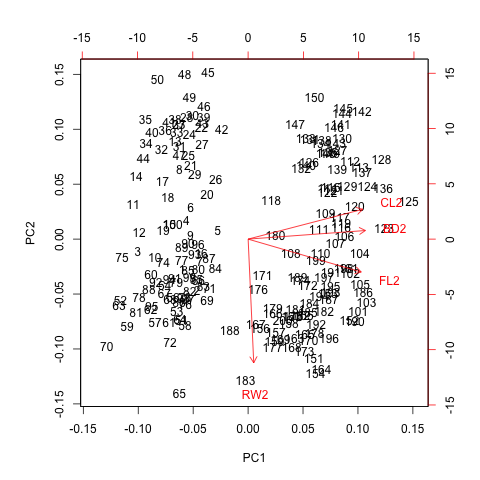
\includegraphics[width=45mm]{Figures/Crabs2_1/plotnospieces.png}
		\captionof{figure}{Représentation des Crabs2 dans les 2 premiers plan factoriel}
		\label{fig:plot_crabs_nocol}
	\end{minipage}%
	\hspace{0.02\linewidth}
	\begin{minipage}{.5\textwidth}
		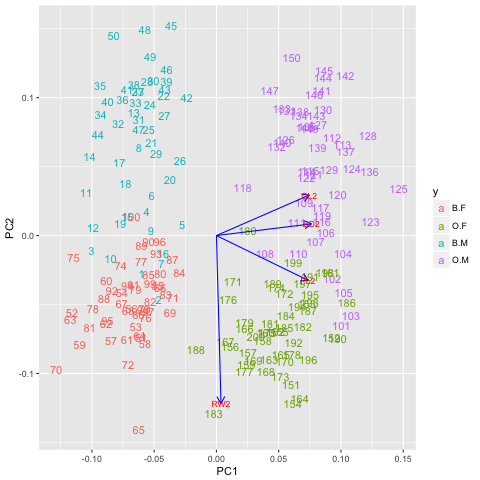
\includegraphics[width=45mm]{Figures/Crabs2_1/plotspieces.png}
		\captionof{figure}{Représentation des  Crabs2 dans les 2 premiers plan factoriel en colorant les espèces}
		\label{fig:plot_crabs}
	\end{minipage}
	\vspace{0.2mm}
	
	Selon la figure \ref{fig:plot_crabs_nocol} on peut observer qu'il existe au moins 2 classes celle de gauche et celle de droite voir 4 classes si on distingue 2 classes dans celle de droite et celle de gauche. Néanmoins on peut remarquer que ces classes ne sont pas très séparées. La figure \ref{fig:plot_crabs} montre qu'il existe bien 4 classes B.F, O.F, B.M et O.M. (B et O pour distinguer les 2 espèces et M et F pour le sexe) . La deuxième composante PC2 qui est concentrée dans la variable RW2 permet de distinguer le sexe, tandis que CL2, FL2, BD2 encodées dans PC1 permettent de distinguer l'espèce.\\ \textbf{On pourrait alors mettre l'hypothèse  que le fait que le sexe ne soit pas aussi distinguable que l'espèce est du au fait qu'il est expliqué que par une seule variable tandis que l'espèce par 3.}
	
	
	\subsection{Mutations}
	Nous disposons dans cette étude  d'une matrice de dissimilarites entre 20 individus (Homme, Singe, Kangourou, Cheval...). Grâce a la méthode \textbf{AFTD} nous allons essayer de réduire la dimension du jeu de données Nous essayerons de trouver au fur et a mesure le bon nombre de variables à choisir.\\ Nous allons alors commencer par réduire le nombre de dimensions à 2. Pour évaluer cette représentations nous utiliserons le pourcentage d'inertie  expliquée cumulée et le  Diagramme de Shepard.  Notons que dans le Diagramme de Shepard un axe représente la disimilarité calculée par l'AFTD alors que l'autre les disimmilarités initiales de la matrice 20x20. Ainsi si la disimilarité calculée par l'AFTD est exacte le Diagramme de Shepard sera une fonction y=x.
	
			\begin{minipage}{.5\textwidth}
		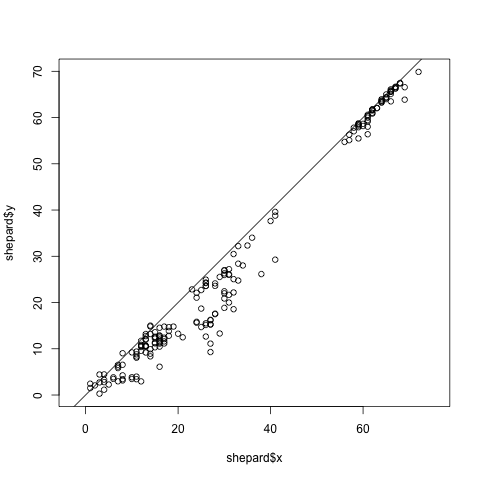
\includegraphics[width=45mm]{Figures/Mutations2_1/shepard2.png}
		\captionof{figure}{Diagramme de Shepard des Mutations avec 2 variables}
		\label{fig:shepard2}
	\end{minipage}%
	\hspace{0.02\linewidth}
	\begin{minipage}{.5\textwidth}
		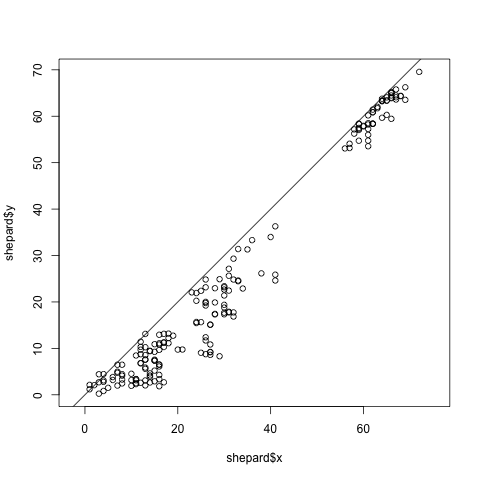
\includegraphics[width=45mm]{Figures/Mutations2_1/shepard3.png}
		\captionof{figure}{Diagramme de Shepard des Mutations avec 3 variables }
		\label{fig:shepard3}
	\end{minipage}
	\vspace{0.2mm}
	
	On remarque d'après les 2 premières présentations ci dessous que le choix de 2 variables n'est pas très représentatif de nos données. En effet les distances calculées par la représentation en 2 dimensions restent loines des distances initiales. Avec 3 variables les disimilarités calculées se rapprochent de leur valeur exacte mais on compte toujours des points éloignés Dans la partie suivante nous allons améliorer cette représentation avec 4 puis 5 variables.
	
		\begin{minipage}{.5\textwidth}
		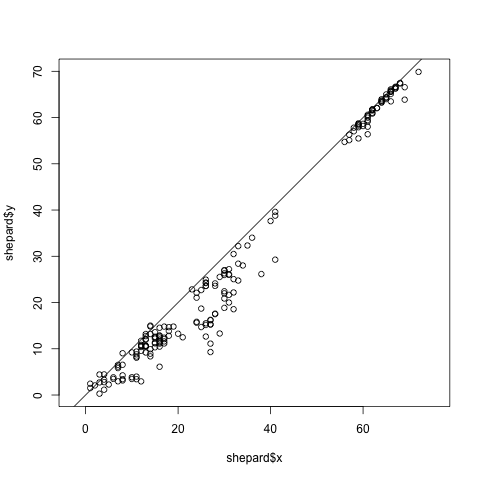
\includegraphics[width=45mm]{Figures/Mutations2_1/shepard4.png}
		\captionof{figure}{Diagramme de Shepard des Mutations avec 4 variables }
		\label{fig:shepard4}
	\end{minipage}%
	\hspace{0.02\linewidth}
	\begin{minipage}{.5\textwidth}
		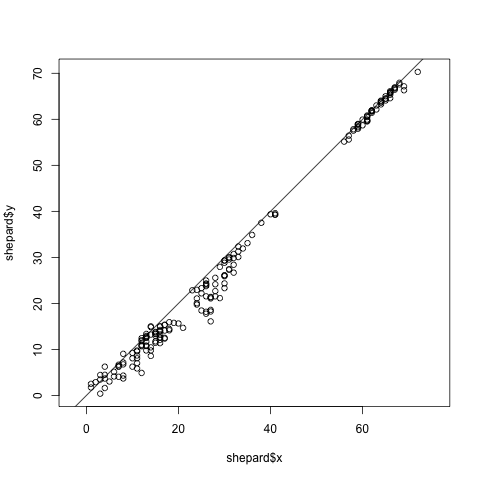
\includegraphics[width=45mm]{Figures/Mutations2_1/shepard5.png}
		\captionof{figure}{Diagramme de Shepard des Mutations avec 5 variables }
		\label{fig:shepard5}
	\end{minipage}
	\vspace{0.1mm}

	Nous remarquons qu' avec 4 variables certaines dissimilarités sont exactes mais d'autres restent fausses. Avec 5 variables on se rapproche plus du cas initial ou toutes les dissimilarités calculées sont plus proche de la droite y=x. Ces résultats étaient prévisibles si on calcule le pourcentage d'inertie expliquée cumulé grâce à l'option \textit{eig = TRUE} dans la fonction \textit{cmscale} pour récupérer les valeurs propres.
	
		\begin{center}
		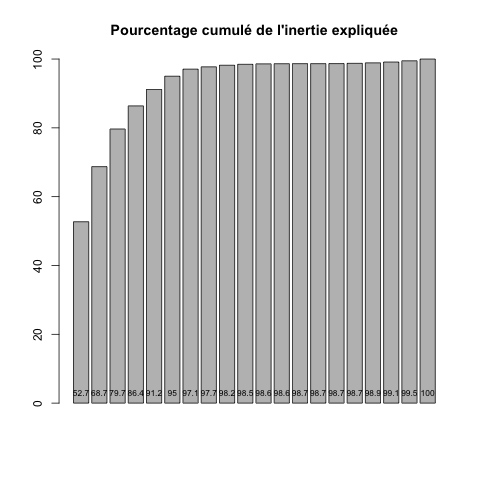
\includegraphics[width=45mm]{Figures/Mutations2_1/barplot.png}
		\captionof{figure}{Pourcentage d'inertie cumulee expliquee par AFTD}
		\label{fig:mutations_barplot}
	\end{center}
	On remarque bien qu'avec 2 variables seulement 68\%  des données sont expliquées et à partir de 4  le pourcentage est supérieur a 86\%.
	
	\subsubsection{Conclusion}
	Pour conclure l'AFTD nous a permis de passer d'une représentation de dissimilarités de dimension 20 à une autre de dimension 5 avec un pourcentage d'inertie expliquée de 91\%. Nous n'avons pas pu choisir 2 dimensions car la représentation n'est pas fiable. On peut supposer que le fait que cette méthode n'a pas été aussi performante avec ce jeu de données est parce que nos dissimilartités ne sont pas des  distances Euclidiennes mais des différences entres les aminos acides dans les chaines chromosomique.
	
	
	

	\section{ Exercice 2: Classification hiérarchique}
	\subsection{Question 1:  Données Mutations}
	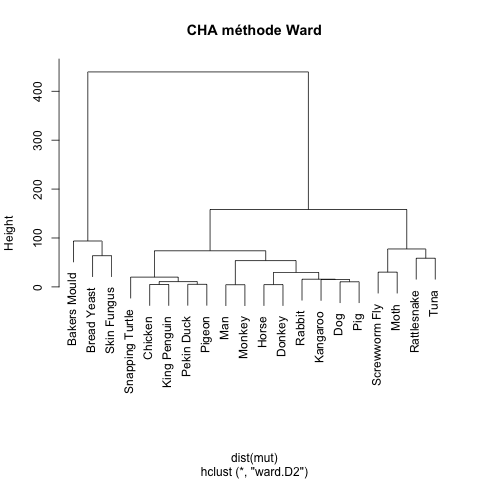
\includegraphics[height = 8cm, width = 8cm]{Figures/HClust/hclust_Mutations_ward.png}
	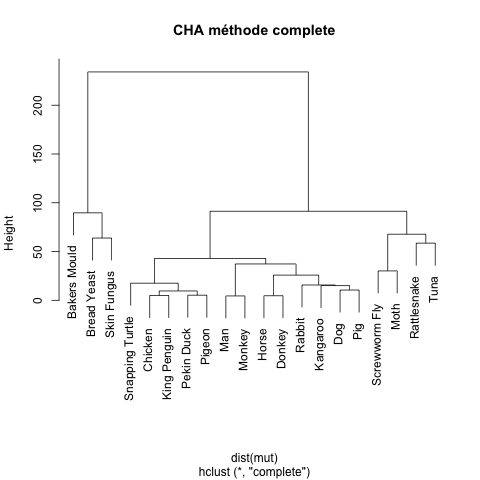
\includegraphics[height = 8cm, width = 8cm]{Figures/HClust/hclust_Mutations_cplt.png}\\
	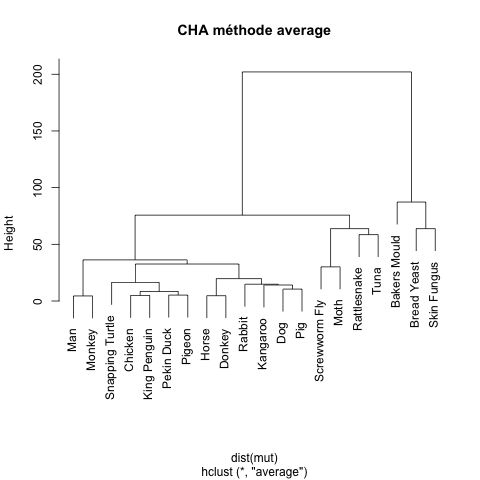
\includegraphics[height = 8cm, width = 8cm]{Figures/HClust/hclust_Mutations_avg.png}
	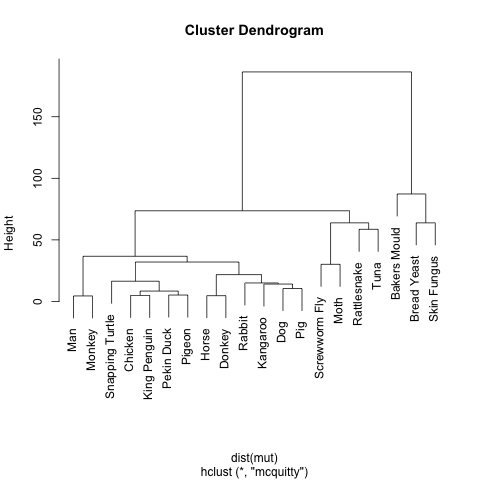
\includegraphics[height = 8cm, width = 8cm]{Figures/HClust/hclust_Mutations_mcq.png}\\
	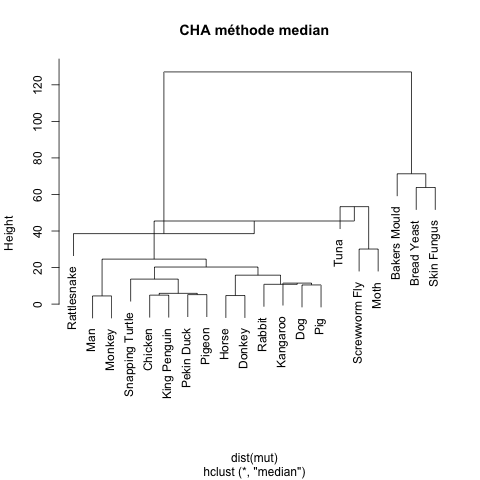
\includegraphics[height = 8cm, width = 8cm]{Figures/HClust/hclust_Mutations_mdn.png}
	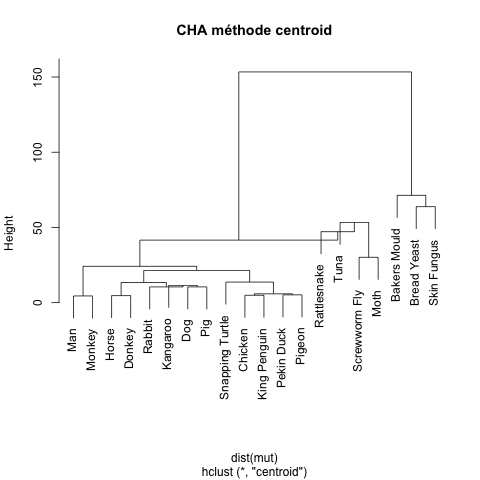
\includegraphics[height = 8cm, width = 8cm]{Figures/HClust/hclust_Mutations_ctr.png}\\
	\begin{center}
		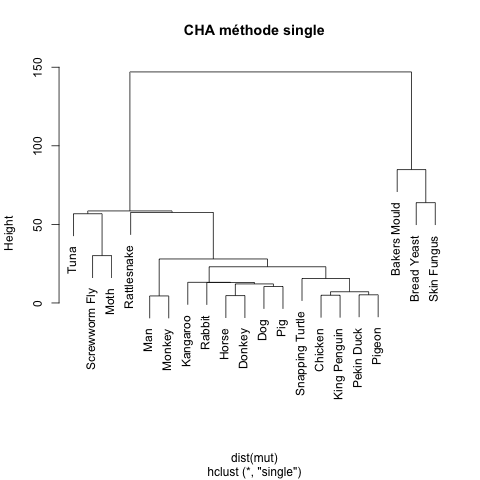
\includegraphics[height = 8cm, width = 8cm]{Figures/HClust/hclust_Mutations_sgl.png}
	\end{center}
	
	Nous remarquons que les méthodes de Ward et complète présentent des CAH identiques. De même la moyenne et Mcquitty d'un autre cote puis la méthode des médianes et des centroides.
	La methode la plus fiable a choisir est celle de Ward car elle minimise les inerties intra-classes des variables quantitatives.

	\subsection{Question 2:  Données Iris (Ascendante)}
	
	Nous utiliserons le critère d'agrégation Ward pour effectuer la classification hiérarchique ascendante des données Iris. Nous mettons en avant aussi les 3 catégories d'espèces.
	\begin{center}
		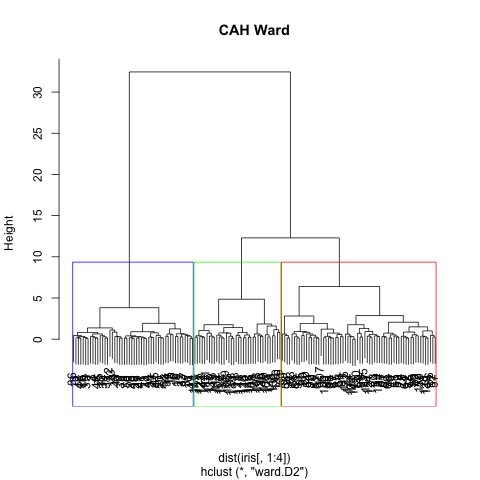
\includegraphics[height = 8cm, width = 8cm]{Figures/HClust/hclust_Iris_ward.png}
	\end{center}

	\begin{minipage}{.5\textwidth}
	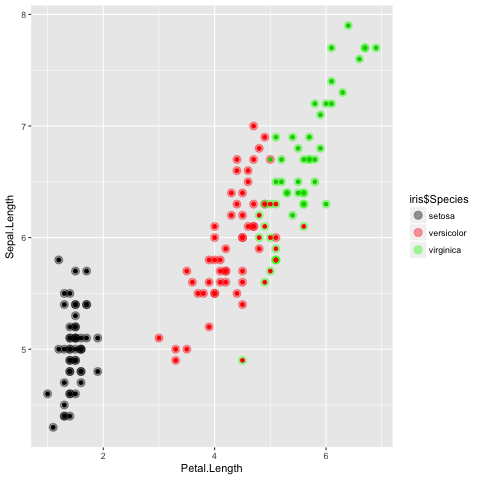
\includegraphics[width = 45mm]{Figures/HClust/ggplot_Iris_ward.png}
	\captionof{figure}{Representation des donnees Iris avec la methode Ward}
	\label{fig:iris_ward_ggplot}
	\end{minipage}%
	\hspace{0.02\linewidth}
	\begin{minipage}{.5\textwidth}
	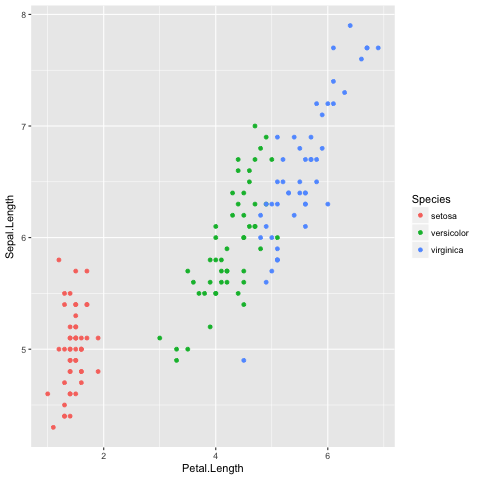
\includegraphics[width = 45mm]{Figures/HClust/ggplot_Iris_normal.png}
	\captionof{figure}{Represenation des donnees normales Iris}
	\label{fig:iris_normal_ggplot}
	\end{minipage}
	\newline
	
	Nous observons grâce au plot le chevauchement des espèces Versicolor et Virginica. Elles sont difficilement différentiables sans couleurs contrairement a l'espèce Setosa.
	
	\subsection{Question 3: Données Iris (Descendante)}
	\begin{center}
		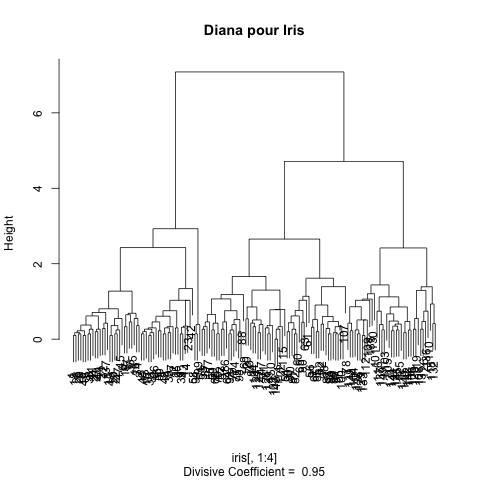
\includegraphics[height = 8cm, width = 8cm]{Figures/HClust/diana_Iris.png}
		\captionof{figure}{Represenation de la classification descendante donnees Iris}
		\label{fig:iris_diana}
	\end{center}
	Nous n'avons pas observe des différences flagrantes entre la classification hiérarchique ascendante et descendante
	
	\section{ Exercice 3: Méthodes des centres mobiles}
	Le but de cet exercice est de manipuler la méthode des kmeans sur les trois jeux de données Iris2, Crabs2 et mutations2 et analyser la qualité de la méthode et ses limites. On utilisera l'index de Rand ajustée ainsi que les représentations graphiques pour juger des performances des kmeans.
	\subsection{Iris2}
	\subsubsection{Question 1}
	Nous commençons par classifier nos méthodes en 2, 3 puis 4 classes et les représenter  en fonction de 2 variables \textbf{Petal.Length et Sepal.Width}. \textbf{Nous avons choisi ces deux variables  car comme on a vu dans la première partie ces dernières sont bien expliquées par les 2 premières composantes principale}s.  Les résultats sont représentés ci-dessous:\\
	
		\begin{minipage}{.5\textwidth}
		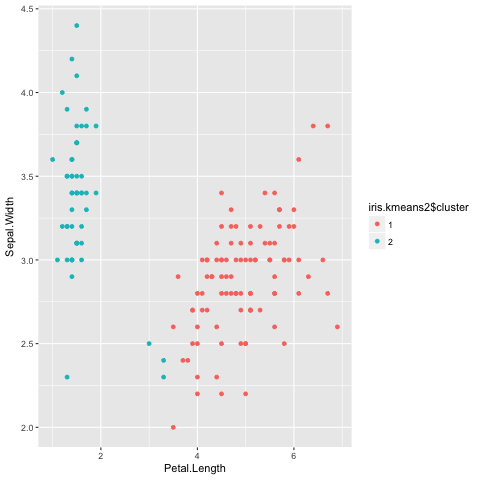
\includegraphics[width=45mm]{Figures/Iris_2/kmeans2.png}
		\captionof{figure}{Representation  de Iris2 en 2 classes}
		\label{fig:iris_kmeans2}
	\end{minipage}%
	\hspace{0.02\linewidth}
	\begin{minipage}{.5\textwidth}
		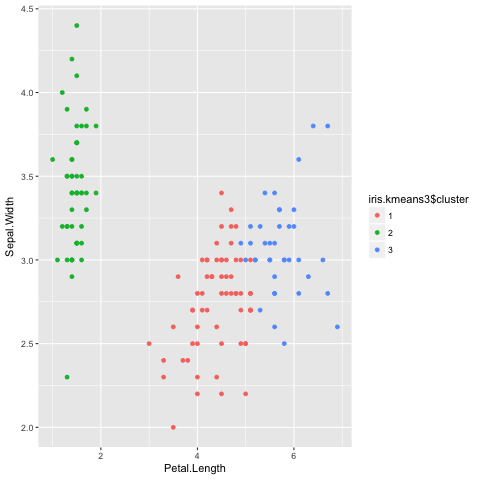
\includegraphics[width=45mm]{Figures/Iris_2/kmeans3.png}
		\captionof{figure}{Representation des Iris2 en 3 classes}
		\label{fig:iris_kmens3}
	\end{minipage}
	\vspace{0.1mm}
	\begin{center}
		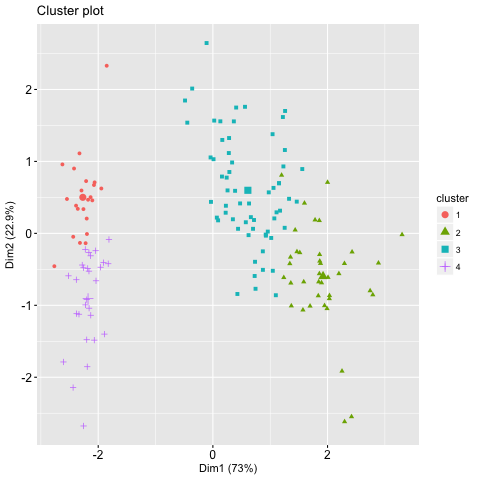
\includegraphics[width=45mm]{Figures/Iris_2/kmeans4.png}
		\captionof{figure}{Representation des Iris2 en 4 classes}
		\label{fig:iris_kmens4}
	\end{center}

On remarque qu'avec \textbf{k= 2 }classes nous obtenons des individus qui appartiennent à la classe 1 alors qu'ils sont plus proche de la classe 2. Tandis qu'avec \textbf{k= 3} on a des individus qui appartiennent à une classe mais qui sont très éloignés La représentation avec \textbf{k= 4} classes semble plus correcte de plus avec une connaissance à priori des données nous savons que c'est le nombre de classe correct.\\


\subsubsection{Question 2}

A présent nous avons effectué plusieurs opérations de kmeans avec k=3, et on remarque qu'à chaque opération nous obtenons des résultats différents. En effet ceci est normal car à la première itération de l'algorithme, celui ci choisit au hasard 3 points (k=3) appartenant aux individus et va construire à partir de ces points les 3 classes. Pour toujours obtenir le même résultat on peut faire un appel  au préalable à la fonction \textit{set.seed(10)} sur R.
	
\subsubsection{Question 3}	
	
Dans cette question nous cherchons à déterminer le nombre de classes minimum dans le jeu de données Iris2. Pour cela on utilise la méthode du coude.  Tout d'abord on effectue 100 opérations kmeans pour chaque k = 2,3...10 en calculant l'\textit{inertie intra-classe}. Ensuite on choisit l'inertie minimum pour représenter l'inertie de chaque k, ce qui s'écrit comme $\hat{I_{k}} = min_{i=1..100} I_{k_{i}}$. Pour cela on utilise une matrice 10*100 ou on sauvegarde l'inertie à chaque opération puis on récupère l'inertie intra-classe minimale de chaque ligne. Le code en R détaillé et commenté de cet algorithme est a trouver en annexe.
La méthode du coude consiste a choisir le point d'inflexion sur la courbe tel que l'inertie intra-classe ne diminue pas de manière aussi rapide en rajoutant des clusters.  Comme il est représenté dans la figure \ref{fig:withinvar}; et comme on s' y attendait aussi, le nombre de classes minimum du jeu de données Iris2 est 3. \\
	
\begin{center}
	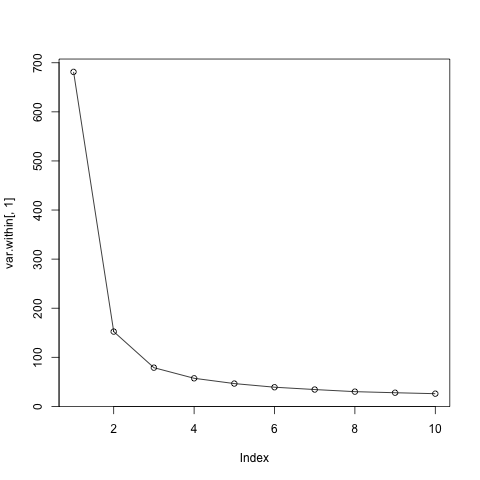
\includegraphics[width=45mm]{Figures/Iris_2/withinvar.png}
	\captionof{figure}{Variation de l'Inertie intra-classe en fonction du nombre de classes}
	\label{fig:withinvar}
\end{center}

 \subsubsection{ Question 4: Analyse des résultats pour k= 3}
Pour analyser la qualité de classification de la méthode des kmeans nous utilisons\textit{ l'index de Rand} ajusté et la représentation graphique. L'indexe de Rand compte le nb de paires de points qui sont classés de la même manière dans les 2 partitions. Cet indice de concordance est calculé en R grâce a la fonction \textit{adjustedRandIndex} . L'index de Rand est compris entre 0 et 1, plus l'index est proche de 1, plus la classification de la méthode correspond à la classification initiale.\

La diagonale de la matrice de confusion représente les points qui sont bien classés. On observe que les individus appartenant à l'espèce \textit{Setosa} sont tous bien classés alors que 96\% des individus de \textit{Versicolor} ont été mal classes et 28\% de \textit{Virginica} sont mal classés aussi.  Nous obtenons un \textbf{index de Rand= 0.73 } ce qui montre que notre classification se rapproche de la vrai classification de la colonne espèces.
Pour pourvoir comparer graphiquement les 2 classement nous avons fait une interaction entre la colonne espèce la colonne \textit{iris.kmeans\$cluster} que nous avons représenté grâce a \textit{ggplot}. 

	\begin{minipage}{.5\textwidth}
		\begin{tabular}{c c c c}	
			Espece &setosa & versicolor & virginica\\
			1     &  50     &     0    &     0\\
			2     & 0       &   2      &  36\\
			3     & 0    &     48   &     14
		\end{tabular}
\end{minipage}%
\hspace{0.08\linewidth}
\begin{minipage}{.5\textwidth}
	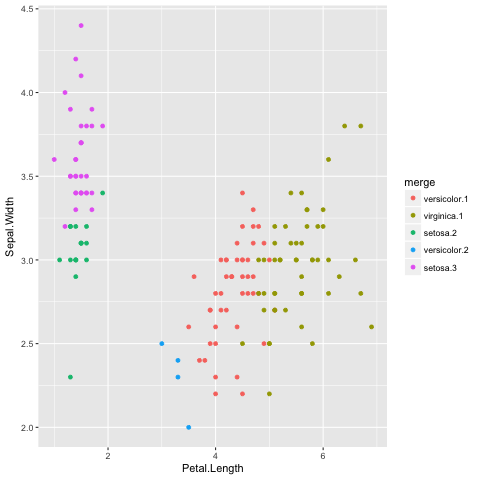
\includegraphics[width=45mm]{Figures/Iris_2/interaction.png}
	\captionof{figure}{Comparaison de la classification originale et celle des kmeans }
	\label{fig:interaction}
\end{minipage}
\vspace{0.1mm}\\

La figure \ref{fig:interaction} rejoint donc bien la remarque faite précédemment comme quoi les espèces \textit{Versicolor} er \textit{Virginica} ne sont pas bien classés. En effet ceci trouve sens si on revient à la figure \ref{fig:plot_iris}, puisqu'on voit bien que l'espèce \textit{Setosa} ne dépend que d'une seule composante PC1 tandis que les 2 autres espèces sont dépendantes des 2 et ne sont pas linéairement séparable.
\subsubsection{Conclusion}
Dans cette exercice nous avons utilisé la méthode des kmeans pour classifier notre jeu de données Iris. Nous retenons que cette méthode est efficace quand on a des classes bien distinctes et linéairement séparables mais n'est pas très flexible.

\subsection{Crabs2}

\subsubsection{Question 1: K=2}

Nous effectuons plusieurs classifications (100 par exemple) des données de Crabs2. Nous remarquons la formations de deux classes essentiellement selon l'espèce comme la figure ci -dessous. Parfois nous obtenons également une classification selon le sexe.
\begin{center}
	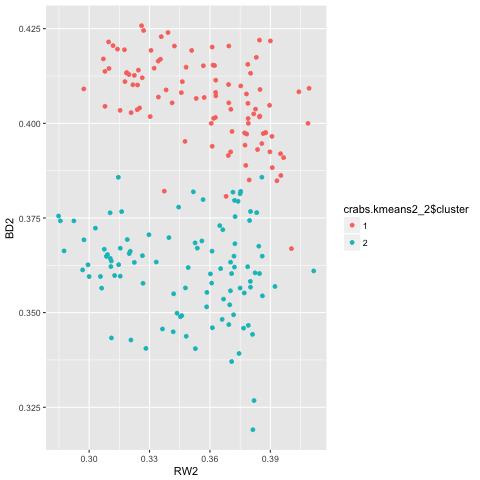
\includegraphics[width=45mm]{Figures/Crabs2_2/kmeans2_1.png}
	\captionof{figure}{Representation  de Crabs2 en 2 classes}
	\label{fig:crabs2_kmeans2}
\end{center}
\hspace{0.02\linewidth}

\subsubsection{Question 2: K=4}

\begin{center}
	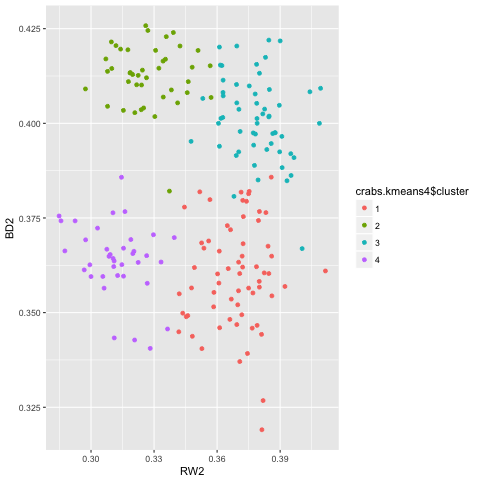
\includegraphics[width=45mm]{Figures/Crabs2_2/kmeans4.png}
	\captionof{figure}{Representation des Crabs2 en 4 classes}
	\label{fig:iris_kmeans4}
\end{center}
\begin{center}
	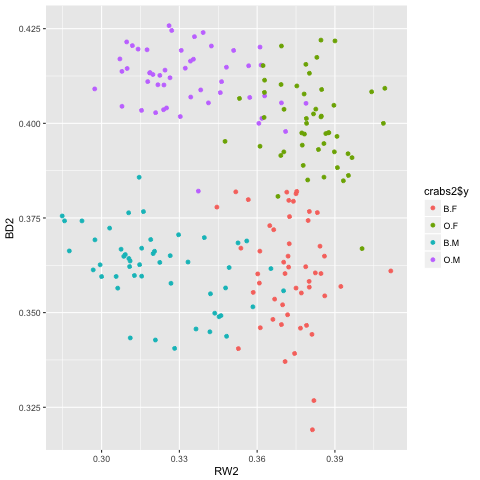
\includegraphics[width=45mm]{Figures/Crabs2_2/plotRealData.png}
	\captionof{figure}{Representation des donnees reelles de Crabs }
	\label{fig:iris_kmeansReal}
\end{center}
En comparant les représentations de la classification en 4 classes et celle des données réelles, nous observons une similitude. Il s'agit de deux classifications en deux classes. Chaque classe représente une combinaison sexe-espèce différente. 

\subsection{Mutations}
Après avoir réalisé l'AFTD pour réduire la dimension de nos jeux de données de 20 à 5, nous utilisons l'algorithme des centres mobiles pour classer les individus en 3 classes. Notons qu'avec 5 variables on explique 91\% des données.\\
Tout d'abord on effectue 1000 itérations en appelant la fonction \textit{kmeans} et on enregistre dans un vecteur l'inertie  intra-classe. Ensuite grâce a la fonction \textit{unique} de R on a pu recensé  6 inerties différentes. Ainsi avec 3 classes on peut classer les espèces de 6 manières différentes. Nous avons représentons ci-dessous 3 de ces classifications.\\

	\begin{minipage}{.32\textwidth}
	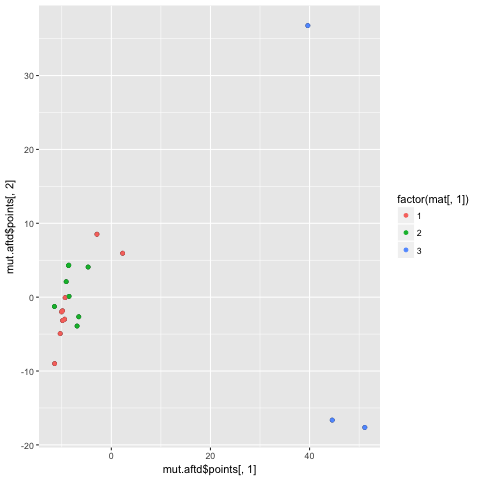
\includegraphics[width=45mm]{Figures/Mutations2_2/kmeans1.png}
	\captionof{figure}{Representation de Mutations2 en 3 classes}
	\label{fig:mutations_kmeans2}
\end{minipage}%
\hspace{0.02\linewidth}
\begin{minipage}{.32\textwidth}
	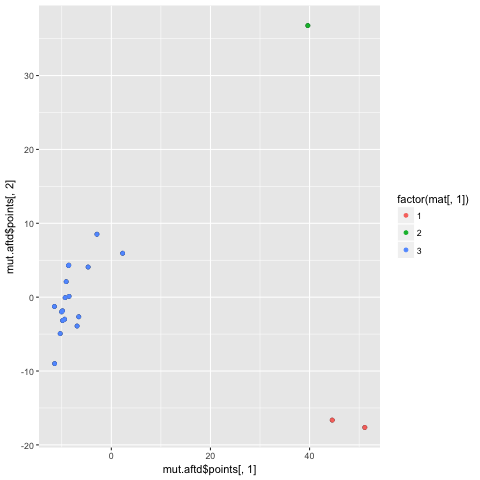
\includegraphics[width=45mm]{Figures/Mutations2_2/kmeans2.png}
	\captionof{figure}{Representation de Mutations2  en 3 classes}
	\label{fig:mutations_kmens3}
\end{minipage}
\begin{minipage}{.32\textwidth}
	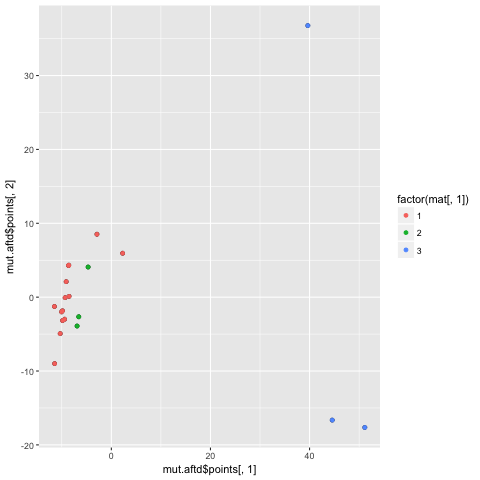
\includegraphics[width=45mm]{Figures/Mutations2_2/kmeans3.png}
	\captionof{figure}{Representation de Mutations2 en 3 classes}
	\label{fig:mutations_kmens4}
\end{minipage}
\vspace{0.02mm}\\
Pour obtenir les différentes classifications il nous a fallu tourner plusieurs fois l'algorithme. C'est aussi une des limites du \textit{kmeans} puisqu'on ne peut pas prédire les résultats, de plus ces derniers peuvent changer d'une itération à l'autre.


\section{Conclusion}
Ce TP nous a permis d'utiliser l'ACP et le AFTD pour réduire les dimensions et classifier les données grâce à l'algorithme des centres mobiles.  L'AFTD semble bien marcher mais elle est plus intéressante à utiliser quand les distances sont Euclidiennes La méthode des centres mobiles est une méthode simple et performante mais n'est pas très flexible quand on a à faire à des classes non linéairement séparables. L'un des gros problèmes de cette méthode est qu'elle fournit des résultats différents.
\end{document}